%%%%%%%% ICML 2019 EXAMPLE LATEX SUBMISSION FILE %%%%%%%%%%%%%%%%%

\documentclass{article}

% Recommended, but optional, packages for figures and better typesetting:
\usepackage{microtype}
\usepackage{graphicx}
\usepackage{subfigure}
\usepackage{booktabs} % for professional tables
\usepackage{amsmath}
\usepackage{amsfonts}
\usepackage{float}
\newcommand{\R}{\mathbb{R}}
\newcommand{\E}{\mathbb{E}}
\newcommand{\Var}{\mathbb{V}\text{ar}}
\newcommand{\Cov}{\mathbb{C}\text{ov}}
\newcommand{\I}{\mathbb{I}}
\newcommand{\Norm}{\mathcal{N}}
\newcommand\given[1][]{\:#1\vert\:}
\newcommand{\bd}[1]{\boldsymbol{#1}}
\newcommand{\hy}{\hat{y}}
\newcommand{\hp}{\hat{p}}
\newcommand{\zbar}{\bar{z}}
\newcommand{\hz}{\hat{z}}
\newcommand{\dbar}{\bar{d}}
\newcommand{\idx}[3][]{{#2}^{(#3)}_{#1}}
\newcommand{\bidx}[3][]{\bd{#2}^{(#3)}_{#1}}

% hyperref makes hyperlinks in the resulting PDF.
% If your build breaks (sometimes temporarily if a hyperlink spans a page)
% please comment out the following usepackage line and replace
% \usepackage{icml2019} with \usepackage[nohyperref]{icml2019} above.
\usepackage{hyperref}

% Attempt to make hyperref and algorithmic work together better:
\newcommand{\theHalgorithm}{\arabic{algorithm}}

% Use the following line for the initial blind version submitted for review:
%\usepackage{icml2019}

% If accepted, instead use the following line for the camera-ready submission:
\usepackage[accepted]{icml2019}

% The \icmltitle you define below is probably too long as a header.
% Therefore, a short form for the running title is supplied here:
\icmltitlerunning{Optimization-Based Approaches for Enforcing Fairness in Machine Learning}

\begin{document}

\twocolumn[
\icmltitle{Optimization-Based Approaches for Enforcing Fairness in Machine Learning}

% It is OKAY to include author information, even for blind
% submissions: the style file will automatically remove it for you
% unless you've provided the [accepted] option to the icml2019
% package.

% List of affiliations: The first argument should be a (short)
% identifier you will use later to specify author affiliations
% Academic affiliations should list Department, University, City, Region, Country
% Industry affiliations should list Company, City, Region, Country

% You can specify symbols, otherwise they are numbered in order.
% Ideally, you should not use this facility. Affiliations will be numbered
% in order of appearance and this is the preferred way.
\icmlsetsymbol{equal}{*}

\begin{icmlauthorlist}
\icmlauthor{Amil Merchant}{equal,harvard}
\icmlauthor{Alexander Lin}{equal,harvard}
\end{icmlauthorlist}

\icmlaffiliation{harvard}{Applied Mathematics 221, Harvard University, Cambridge, Massachusetts, USA}

\icmlcorrespondingauthor{Amil Merchant}{amilmerchant@college.harvard.edu}
\icmlcorrespondingauthor{Alexander Lin}{alexanderlin01@college.harvard.edu}

% You may provide any keywords that you
% find helpful for describing your paper; these are used to populate
% the "keywords" metadata in the PDF but will not be shown in the document
\icmlkeywords{Machine Learning, ICML}

\vskip 0.3in
]

% this must go after the closing bracket ] following \twocolumn[ ...

% This command actually creates the footnote in the first column
% listing the affiliations and the copyright notice.
% The command takes one argument, which is text to display at the start of the footnote.
% The \icmlEqualContribution command is standard text for equal contribution.
% Remove it (just {}) if you do not need this facility.

%\printAffiliationsAndNotice{}  % leave blank if no need to mention equal contribution
\printAffiliationsAndNotice{\icmlEqualContribution} % otherwise use the standard text.

\begin{abstract}
	Machine learning methods are increasingly being used to make decisions of large social consequence, including credit scoring and recidivism prediction. Although the predictive power of these models is impressive, the data used to train them often contains historical prejudices. This leads to unfair predictions and discrimination based on sensitive attributes such as race or sex. In this paper, we consider two flexible mechanisms to minimize the disparities in predictions between groups. The first extends previous literature on fairness constraints, whereas the second uses an adversarial approach to equalize score distributions between groups. We test both methods on the adult income dataset and find that both lead to fair classifiers without sacrificing significant accuracy.
\end{abstract}

\section{Introduction}
\label{submission}

Over the past few years, machine learning (ML) and artificial intelligence (AI) have become increasingly more common for high-stakes decision making.  Researchers have proposed machine learning algorithms for applications such as credit scoring \citep{huang2007credit}, personalized medicine \citep{poplin2018prediction}, and redicivism prediction \citep{tollenaar2013method}.  

In light of our increased adoption of ML/AI methods, it is important that we do not allow these technologies to foster unfairness within our society.  Machine learning algorithms fundamentally rely on past data in order to function.   They attempt to generalize patterns found in the data and apply these patterns to make predictions in future scenarios.  However, in certain situations, historical injustices against presently protected subgroups of a population may have led to the recording of biased data.  Naively training a model on this biased data may lead to a biased algorithm that discriminates against these protected subgroups.  Subsequently using this algorithm for high-stakes decision making may lead to further injustices and bias the collection of future data, thereby leading to a dangerous positive feedback loop.  

Thus, finding ways to enforce fair predictions for machine learning algorithms is a problem of utmost importance.  In this paper, we propose and test some methods that strive to achieve this goal.  These methods are primarily optimization-based, meaning that they each involve augmenting the objective function of machine learning methods in some manner and can be seen as a form of regularization.  We employ our methods in neural networks, models that have garnered a great deal of popularity in recent years due to empirical success across many domains.  Our empirical results are presented on the \emph{adult income dataset}\footnote{This dataset is publicly available at \url{https://archive.ics.uci.edu/ml/datasets/adult}.}, which was collected from 1994 census data \citep{kohavi1996scaling}.  We show that our proposed approaches can significantly reduce model bias defined in the form of \emph{disparate impact} and uphold desired levels of \emph{demographic parity} without sacrificing a prohibitive amount of accuracy.             

\subsection{Related Work}
Recently, there has been an increasing focus on satisfying fairness in a machine learning context. The rise of this field corresponded to widespread concern about a model known as COMPAS. Used in the justice system of the United States to forecast recidivism probabilities, the predictions are used by judges to determine whether defendants receive bail, lighter sentences, or even early parole. While the predictive power of the model was impressive, \citet{angwin2016machine} showed that the model has a discriminatory impact on African-American defendants compared to their Caucasian counterparts. 

Within the computer science literature, a number of papers have introduced new fairness criterion to quantitatively measure the differential effects of these machine learning models. For example, \citet{hardt2016equality} argued for equalizing the True Positive and False Positive Rates between protected groups in a metric known as equality of odds. \citet{kusner2017counterfactual} have proposed a more causal definition of fairness known as counterfactual fairness. In a recent review, \citet{narayanan} summarized 21 different definitions of fairness and the social implications of each. In this paper, we focus on one of the first proposed and arguably one of the simplest fairness criteria, known as demographic parity. This definition is particularly interesting due to its legal implications for showing that a model is discriminatory.

Similarly, a number of approaches have been developed to minimize the differences between individuals based on race, gender, etc. Some of the earliest strategies involved pre-processing the available data to learn a representation space where the differences are minimized. \citet{dwork2012fairness} and  \citet{feldman2015certifying} utilized such approaches. However, these methods struggled with unpredictable and large losses in accuracy in order to ensure fairness. This paper follows two more recent research directions: introducing constraints and adversarial learning.

Instead of focusing on the inputs, constraint-based learning introduced regularization terms for classifiers to ensure fairness. For example, \citet{kamishima2012fairness} introduced a penalty to correct the training of logistic regression classifiers. More recently, \citet{zafar2015fairness} introduced a generalizable method by penalizing properties of the decision boundary.

Adversarial networks have been utilized by a number of papers to enforce fairness definitions. For example, \citet{beutel2017data} shared hidden layers between various networks to enforce demographic parity. More recently, \citet{wadsworth2018achieving} introduced the setup of a predictor attempting to maximize accuracy and an adversary enforcing fairness.

In this paper, we extend the methods of \citet{zafar2015fairness} and \citet{wadsworth2018achieving} to create fair classifiers that are able to ensure fairness without forsaking significant accuracy.

\section{Background}

\subsection{Adult Income Dataset}

The adult income dataset \citep{kohavi1996scaling} contains data from $N = 32,561$ respondents to the 1994 United States Census.  Each person $n$ is characterized by $J = 14$ attributes, denoted $\bidx x n = \{\idx[1] x n, \ldots, \idx[J] x n\}$, including education level, occupation type, capital gains, capital losses, and number of hours worked per week.  The goal is to predict a binary variable $\idx y n \in \{0, 1\}$, which indicates whether or not person $n$ makes over \$50,000 a year.

In this case, the protected attributes $\bidx z n$ for person $n$ are their \emph{sex} and their \emph{race}.  Historical inequities have led to groups such as women and African Americans having significantly lower fractions of individuals making over \$50,000 a year.  Using a model naively trained on the adult income dataset for high stakes decision making in the present day -- such as estimating a person's income for loan approval or determining how much to pay a new hire -- may lead to heavily biased results.  Thus, there is motivation to incorporate predictive fairness into the model training process.

\subsection{Disparate Impact and Demographic Parity}   

\emph{Disparate impact} is the notion in which a model's biased classification process leads to outcomes that disproportionately hurt (or benefit) people with sensitive attributes.  It was first introduced by \citet{zafar2015fairness}.  Simply removing the sensitive attributes $\bd z$ from the dataset and training a model on the remaining attributes $\bd x \setminus \bd z$ may still yield biased predictions, because $\bd z$ may be correlated with the remaining subset \citep{agarwal2018reductions}.

To counter disparate impact, we wish to enforce \emph{demographic parity}, which demands that the distribution of scores for any protected classes is the same.  Let $\hat{p}(y = 1)$ be a model's prediction of the probability of class 1 in binary classification.  Formally, demographic parity is defined as:
\begin{align}
\hp(y = 1 \given \bd z = k_1) = \hp(y = 1 \given \bd z = k_2),
\end{align}  
where $k_1$ and $k_2$ are different realizations of the random variable $\bd z$.  For example, if $\bd z$ is sex, $k_1$ could be \texttt{Male} and $k_2$ could be \texttt{Female}.  Intuitively, this means that only changing the protected attribute $\bd z$ should not influence the predictions in any way.  

Using demographic parity as a definition of machine learning fairness offers some advantages.  First and foremost, there exists legal support for this definition in the United States.  In 1978, four government agencies -- including the EEOC, Department of Labor, Department of Justice, and the Civil Service Commission -- proposed the four-fifths (or 80\%) rule as a benchmark with assessing adverse disparate impact for protected classes \citep{bobko2004four}.  Specifically, these agencies required that
\begin{align}
\min \left\{\frac{\hp(y = 1 \given \bd z = k_1)}{\hp(y = 1 \given \bd z = k_2)}, \frac{\hp(y = 1 \given \bd z = k_2)}{\hp(y = 1 \given \bd z = k_1)} \right\} \geq \frac{q}{100} \label{q-rule}
\end{align} 
where $q = 80$ in the legal definition.  Note that $q = 100$ corresponds to zero disparate impact and complete demographic parity.  Recently, \citet{hu2018short} additionally argue that short-term enforcement of demographic parity has long-term benefits for countering discrimination against minorities in the labor market.  

\section{Methods for Enforcing Demographic Parity}
We present two optimization-based methods for enforcing demographic parity in neural networks.  

A neural network is a cascade of linear and nonlinear transformations of the input vector $\bd x$ to yield an output vector $\bd h_L$ \citep{goodfellow2016deep}.  An $L$-layer neural network can be described by the equations,
\begin{align}
\bd h_1 &= \idx f {1}(\idx W {1} \bd x + \idx b {1}), & \quad \ldots  \label{nn-def} \\
\bd h_\ell &= \idx f {\ell}(\idx W {\ell} \bd h_{\ell - 1} + \idx b {\ell}), & \quad \ldots\nonumber \\
\bd h_L &= \idx f {L}(\idx W {L} \bd h_{L-1} + \idx b {L}), \nonumber
\end{align}  
where each pair $(\idx W \ell, \idx b \ell)$ parameterizes an affine transformation (via matrix multiplication and bias addition), each $\idx f \ell$ is a nonlinear function applied element-wise, and each $\bd h_\ell$ denotes an intermediary hidden state representation of the input.  

In binary classifiers, it is common to let $\idx W L$ be a row vector, $\idx b L$ be a single scalar, and $\idx f L$  be the sigmoid function $\sigma(a) = 1 / (1 + \exp (- a))$.  Such constraints force the final output $\hat{p} = \bd h_L$ to be a scalar within the range $[0, 1]$, which allows us to interpret it as the estimated probability of $y = 1$.  For selected nonlinearities $\{\idx f \ell\}_{\ell=1}^L$, the weights $\{\idx W \ell\}_{\ell=1}^L$ and biases $\{\idx b \ell\}_{\ell=1}^L$ are trained to minimize the \emph{binary cross-entropy loss} $Q_0$ over the entire dataset, which is defined as
\begin{align}
Q_0 = \sum_{n=1}^N \idx y n \log \idx \hp n + (1 - \idx y n) \log (1 - \idx \hp n), \label{bce}
\end{align}         
where each $\idx \hp n$ is generated by passing $\bidx x n$ through the neural network.

\subsection{Regularizing Decision Boundary Covariance} \label{method1}
\citet{zafar2015fairness} propose regularizing the covariance between the distance to the decision boundary of a classifier and the protected classes $\bd z$ to enforce demographic parity.  They apply their framework to logistic regression and support vector machines.  We generalize this method to working with neural networks.

Using the neural network binary classifier of Equation \ref{nn-def}, we define the \emph{decision boundary distance} $\idx d n$ of training example $n$ as the value obtained before the final nonlinearity, i.e. 
\begin{align}
\idx d n = \idx W {L} \bidx[L-1] h n + \idx b {L}. \label{decision-boundary-def}
\end{align} 
To see why $\idx d n$ is related to the decision boundary of the neural network classifier, observe that the estimated probability of $\idx y n = 1$ is $\idx \hp n = \sigma(\idx d n)$.  Thus, if $\idx d n > 0$, then $\idx \hp n > 1/2$ (so it makes more sense to classify $n$ as class 1) and if $\idx d n < 0$, then $\idx \hp n < 1/2$ (so it makes more sense to classify $n$ as class 0).  Thus, the variable $d$ encodes a scale centered at zero and characterizes the confidence of the classifier to classify as class 0 or class 1.  

If the covariance between the decision boundary distance $d$ and the protected attribute $\bd z$ is zero, then knowing $\bd z$ should have no impact on knowing $p(y \given \bd x)$, which is the definition of satisfying demographic parity.  We can empirically estimate this covariance by observing the following:
\begin{align}
\Cov(\bd z, d) &= \E[(\bd z - \bd \zbar) \cdot (d - \dbar)] \\
&= \E[(\bd z - \bd \zbar) \cdot d] - \E[(\bd z - \bd \zbar)] \cdot \dbar \nonumber \\
&= \E[(\bd z - \bd \zbar) \cdot d] - 0 \nonumber \\
&\approx \frac{1}{N} \sum_{n=1}^N (\bidx z n - \bd \hz) \cdot \idx d n, \nonumber
\end{align}      
where $\bd \hz = 1 / N \cdot \sum_{n=1}^N \bidx z n$.  Since \citet{zafar2015fairness} work with only convex classifiers, they simply add the following convex constraint to their logistic regression and support vector machine settings:
\begin{align}
\left | \frac{1}{N} \sum_{n=1}^N (\bidx z n - \bd \hz) \cdot \idx d n \right | \leq \bd c,
\end{align}
for some constant $\bd c$ corresponding to the level of desired demographic parity.  In our neural network setting, we instead directly add the empirical covariance as a penalized regularization term to the binary cross entropy objective function of Equation \ref{bce}.  Thus, the full objective function is
\begin{align}
Q_1 &= \sum_{n=1}^N \idx y n \log \idx \hp n + (1 - \idx y n) \log (1 - \idx \hp n) \label{penalty-bce} \\ 
&\quad + \lambda \cdot \left | \frac{1}{N}  \sum_{n=1}^N (\bidx z n - \bd \hz) \cdot \idx d n \right|, \nonumber
\end{align}
where $\lambda$ controls the degree of regularization.  Increasing $\lambda$ will increase the penalty of the covariance and ideally lead to greater demographic parity.  We wish to adjust $\lambda$ so that it is large enough to satisfy fairness constraints, yet small enough to not prohibitively affect classifier accuracy.    

\subsection{Regularizing with Adversarial Networks}
\label{sec:adversarial} 

Adversarial networks were first introduced by \citet{goodfellow2014generative} in the context of generative adversarial nets, which simulate a minimax two-player game between two neural networks.  The \emph{generator} attempts to create realistic-looking fake images, while the \emph{discriminator} attempts to distinguish real images from fake ones.  The generator is trained so that the discriminator (also known as the \emph{adversary}) performs poorly, which allows the generator to reach an equilibrium in which the distribution of its synthesized images approximates that of the training set. 

\citet{wadsworth2018achieving} apply the idea of adversarial networks to fairness in machine learning, specifically looking at the context of criminal recidivism prediction.  We use this concept in our income prediction problem.  

Let $G$ be a neural network binary classifier (Equation \ref{nn-def}) that optimizes for binary cross-entropy loss $Q_0$ (Equation \ref{bce}).  Define the logit of the output probability for training example $n$ as $\idx d n = \sigma^{-1}(\idx \hp n)$, where $\sigma$ is the sigmoid function; notice that this is equivalent to the decision boundary distance of Equation \ref{decision-boundary-def}.  We train a second neural network binary classifier $A$, known as the discriminator (or adversarial network), that learns to classify the sensitive attribute $\bd z$ using $d$.  That is, $A$ works with the supervised training set $\{(\idx d 1, \bidx z 1), \ldots, (\idx d N, \bidx z N)\}$.  Its loss function also follows the form of binary cross-entropy:    
\begin{align}
Q_A = \sum_{n=1}^N \bidx z n \log A(\idx d n) + (1 - \bidx z n) \log (1 - A(\idx d n)). \label{bce}
\end{align}         

Then, in the spirit of generative adversarial networks, $G$ is trained so that $A$ performs poorly.  In other words, the augmented loss function of $G$ is:
\begin{align}
Q_2 = Q_0 - \alpha \cdot Q_A,
\end{align}
where $\alpha \geq 0$ controls the tradeoff between optimizing for $Q_0$ versus $-Q_A$.  In the case where the loss function $Q_A$ reaches its maximum, there is no way to predict the sensitive attribute $\bd z$ from the output of $G$, which implies zero disparate impact and complete demographic parity.   

\citet{goodfellow2014generative} provide some theoretical results that show the concept of adversarial training aims to minimize the Jensen-Shannon divergence $\mathbb{JS}$ between two probability distributions $q_1$ and $q_2$.  This is given as
\begin{align}
\mathbb{JS}(q_1, q_2) = \frac{1}{2} \mathbb{KL}\left(q_1 || q_{12}\right) + \frac{1}{2} \mathbb{KL}\left(q_2 || q_{12} \right),
\end{align}    
where $q_{12} = (q_1 + q_2) / 2$ and $\mathbb{KL}$ denotes the Kullback-Leibler divergence.  The Jensen-Shannon divergence has some nicer properties, such as symmetry, in comparison to other similar divergences in its family.  

In the case of fairness, these distributions are the conditional distributions $d \given \bd z = k_1$ and $d \given \bd z = k_2$ output by $G$ for the logit output probabilities $d$ with respect to the sensitive attribute $\bd z$.  Through the deterministic sigmoid transformation $\sigma$, we arrive at prediction probabilities $\hp(y = 1 \given \bd z = k_1)$ and $\hp(y = 1 \given \bd z = k_2)$, respectively.  In our application, it makes sense to constrain these distributions to be close to one another, because the very definition of demographic parity (Equation \ref{q-rule}) is tied to this fact.          

\section{Results}
Our empirical results are evaluated on the adult income dataset.  We first naively train a vanilla neural network and show how it suffers from disparate impact.  Then, we apply our methods for enforcing demographic parity to exhibit how this disparate impact can be mitigated.  All experiments are implemented using the PyTorch deep learning library \citep{paszke2017pytorch}.  

\subsection{Vanilla Neural Network} \label{vanilla-net}

We train a simple neural network with $L = 2$ layers that performs well on the adult income dataset.  The input is $\bd x \setminus \bd z$, the set of all attributes minus sex and race.  The single hidden layer $\bidx h 1$ has 64 hidden units.  We let $\idx f 1$ be the rectified linear (ReLU) function and $\idx f 2$ be the sigmoid function.  Weights and biases $\{\idx W 1, \idx W 2, \idx b 1, \idx b 2\}$ are initialized as $\mathcal{N}(0, 1)$ random variables.  

We divide the dataset of $N = 32,561$ individuals into a training set $\mathcal{D}_\text{train}$ of $26,048$ people and test set $\mathcal{D}_\text{test}$ of $6,513$ people, which roughly corresponds to an 80\%-20\% split.  The network is trained using the binary cross entropy loss function of Equation \ref{bce} on $\mathcal{D}_\text{train}$.  For optimization, we use the ADAM stochastic optimizer \citep{kingma2014adam} with a minibatch of $1,024$ examples.  The network is trained for 20 epochs, which are defined as passes through the entire training set.   

Evaluation is performed on the test set.  Test set accuracy is 85.00\%, which is decent.  However, there are gross violations of demographic parity.  

If we observe the distributions over estimated probabilities of making over 50K divided by sex (i.e. \texttt{Male} vs. \texttt{Female}), we see that there are significant discrepancies.  Figure \ref{vanilla-nn} traces the distribution of $\idx \hp n \given \bidx z n = \texttt{Male}$ and $\idx \hp n \given \bidx z n = \texttt{Female}$ for all $n \in \mathcal{D}_\text{test}$ by using simple kernel density estimation.  The shapes are quite different.  Let $\mathcal{D}_\text{test}^\texttt{Male}$ and $\mathcal{D}_\text{test}^\texttt{Female}$ be partitions of $\mathcal{D}_\text{test}$ based on sex.  We see that the largest possible $q$ that satisfies Equation \ref{q-rule} is $q = 41.82\%$, where $q$ is found empirically in this example as 
\begin{align}
q = \frac{| \mathcal{D}_\text{test}^\texttt{Female} |^{-1} \sum_{n \in \mathcal{D}_\text{test}^\texttt{Female}} \idx \hp n}{| \mathcal{D}_\text{test}^\texttt{Male} |^{-1} \sum_{n \in \mathcal{D}_\text{test}^\texttt{Male}} \idx \hp n}.
\end{align} 

This model exhibits significant bias against females, likely because it was trained on a biased dataset.  Thus, it is unsuitable for use in future high-stakes decision making, such as determining how much a female should make or estimating a female's income for loan approval. 

We can repeat the same exercise for race on analogously defined datasets $\mathcal{D}_\text{test}^\texttt{Minorities}$ and $\mathcal{D}_\text{test}^\texttt{White}$.  For race, we find that $q = 63.63\%$, which is less unfair, yet still violates the 80\% rule used in legal settings.  Figure \ref{vanilla-nn} presents the corresponding plot.

Mean predicted probabilities of high-income for the aforementioned sensitive groups can be found in Table \ref{vanilla-table}.

\begin{figure}[ht]
\vskip 0.2in
\begin{center}
\centerline{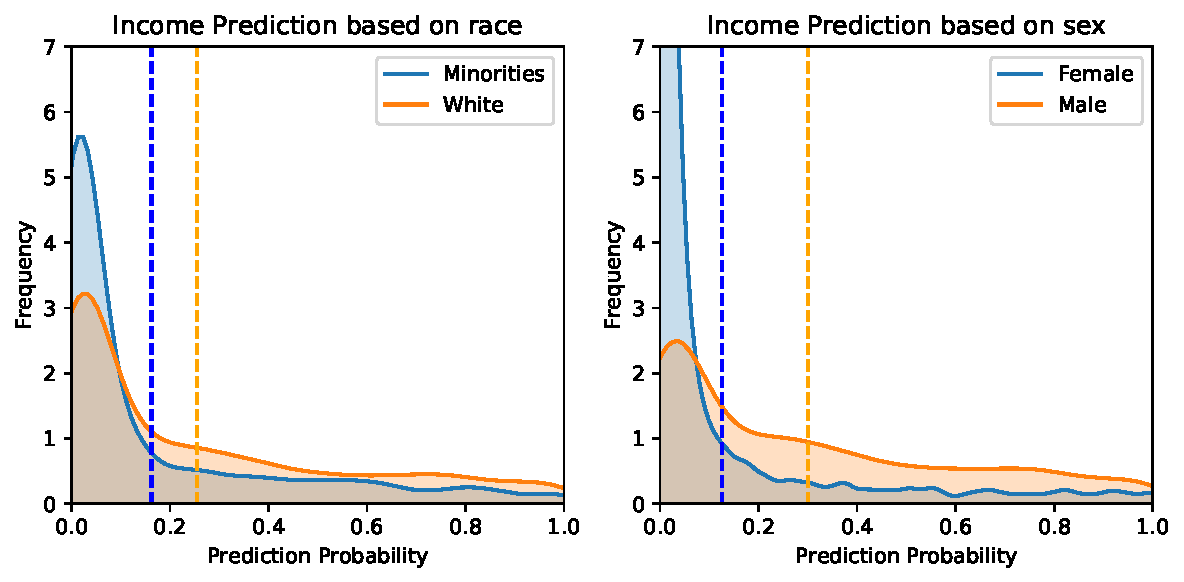
\includegraphics[width=\columnwidth]{img/vanilla-bias.pdf}}
\caption{For the vanilla neural network, fitted kernel density estimations of test set estimated probabilities that different races (left) and different sexes (right) make over 50K a year.  Dotted lines indicate the means of each distribution (Table \ref{vanilla-table}).}
\label{vanilla-nn}
\end{center}
\vskip -0.2in
\end{figure}

\begin{table}[h]
\centering
\begin{tabular}{c|c||c |c} 
 \hline
 Female & Male & Minorities & White \\ [0.5ex] 
 0.125 & 0.300 & 0.162 & 0.256 \\
 \hline
\end{tabular}
\caption{For the vanilla neural network, test set mean estimated probabilities of making over 50K for various sensitive groups.} \label{vanilla-table}
\end{table}

\subsection{Regularizing Decision Boundary Covariance}

We apply the method described in Section \ref{method1} to correcting disparate impact for the vanilla neural network of Section \ref{vanilla-net}.  In doing so, we keep the same general architecture and training hyperparameters described in the previous section.  However, instead of training the network using normal binary cross-entropy loss $Q_0$  (Equation \ref{bce}), we instead use the regularized objective $Q_1$ that penalizes decision boundary covariance (Equation \ref{penalty-bce}).  

In our experiments, we vary the regularization penalty $\lambda$ to show corresponding effects on the final accuracy and fairness of the neural network classifier.  We try $\lambda$ within the set $\{3 \times 10^{-2}, 1 \times 10^{-2}, 3 \times 10^{-3}, 1 \times 10^{-3}, 3 \times 10^{-4}, 1 \times 10^{-4}\}$, which covers approximate increases in factors of three.  

Graphs and a table of the results for sex on the training and test sets can be found in Figure \ref{boundary-fig-sex} and Table \ref{boundary-table-sex}, respectively.  We see that choosing a suitable $\lambda$ can satisfy demographic parity without sacrificing significant amounts of accuracy.  Looking at Figure \ref{boundary-fig-sex} and Table \ref{boundary-table-sex}, there is a sharp bend in the curve for $\lambda = 3 \times 10^{-3}$, so this is an appropriate final choice.

Similar results for race can be found in Figure \ref{boundary-fig-race} and Table \ref{boundary-table-race}.  Looking at these values, it appears that $\lambda = 1 \times 10^{-3}$ is a reasonable choice here.  

Figure \ref{boundary-bias} shows the effect of regularizing the network on aligning the prediction distributions for the sensitive attributes using the aforementioned values of $\lambda$.  Comparing this graph with Figure \ref{vanilla-nn}, we see that the gains in demographic parity are significant.  The tables also show that the test accuracy for our chosen values of $\lambda$ drop by a maximum of $1.2\%$, which is very little in comparison.

\begin{figure}[ht]
\vskip 0.2in
\begin{center}
\centerline{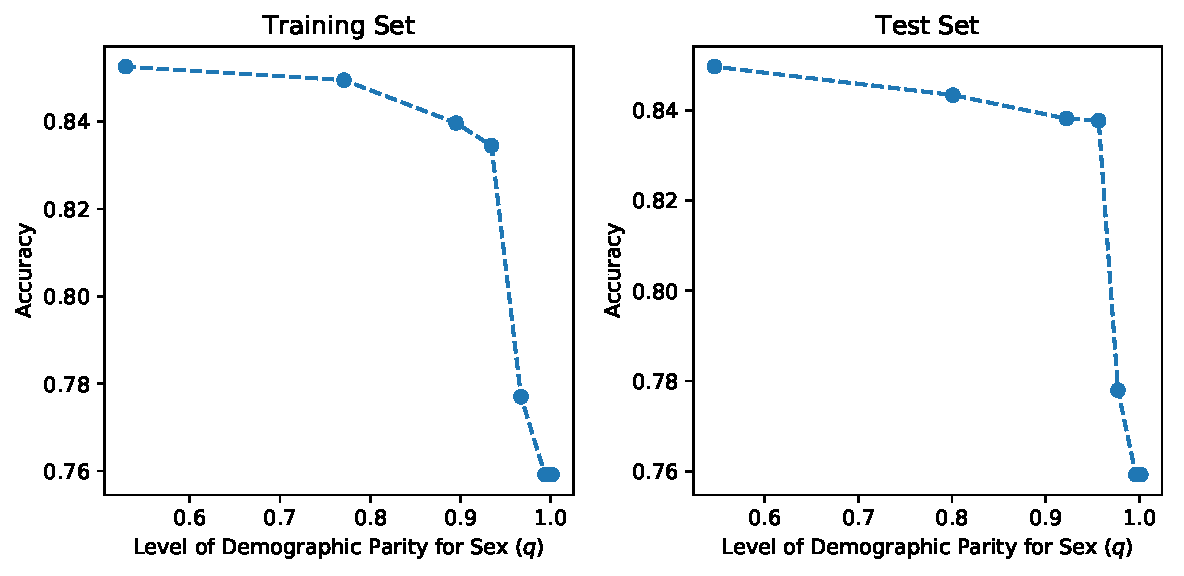
\includegraphics[width=\columnwidth]{img/boundary-tradeoff-sex.pdf}}
\caption{Tradeoff between overall neural network accuracy and level of demographic parity for \emph{sex} by varying regularization penalty $\lambda$ on the covariance between the distance to the decision boundary and sensitive attributes.  Results are given on the training set (left) and the test set (right).}
\label{boundary-fig-sex}
\end{center}
\vskip -0.2in
\end{figure}

\begin{table}[ht]
\centering
\begin{tabular}{c|cc |cc} 
 \hline
 \hline
 $\lambda$ (for Sex) & Train Acc & Train $q$ & Test Acc & Test $q$ \\ 
 \hline
 $3 \times 10^{-2}$ & 0.759 & \textbf{0.994} & 0.759 & \textbf{0.996}\\
 $1 \times 10^{-2}$ &0.777& 0.967 & 0.778 & 0.977\\
$3 \times 10^{-3}$ & 0.834 & 0.934 & 0.838 & 0.957 \\
$1 \times 10^{-3}$ & 0.840 & 0.895 & 0.838 &0.922 \\
$3 \times 10^{-4}$ & 0.849 & 0.771 & 0.843 & 0.801\\
$1 \times 10^{-4}$ & \textbf{0.852} & 0.529 & \textbf{0.850} & 0.547\\
 \hline
\end{tabular}
\caption{Numerical results of how accuracy and level of demographic parity change as functions of regularization parameter $\lambda$ for constraining prediction probabilities conditioned on \emph{sex}.} \label{boundary-table-sex}
\end{table}

\begin{figure}[!ht]
\vskip 0.2in
\begin{center}
\centerline{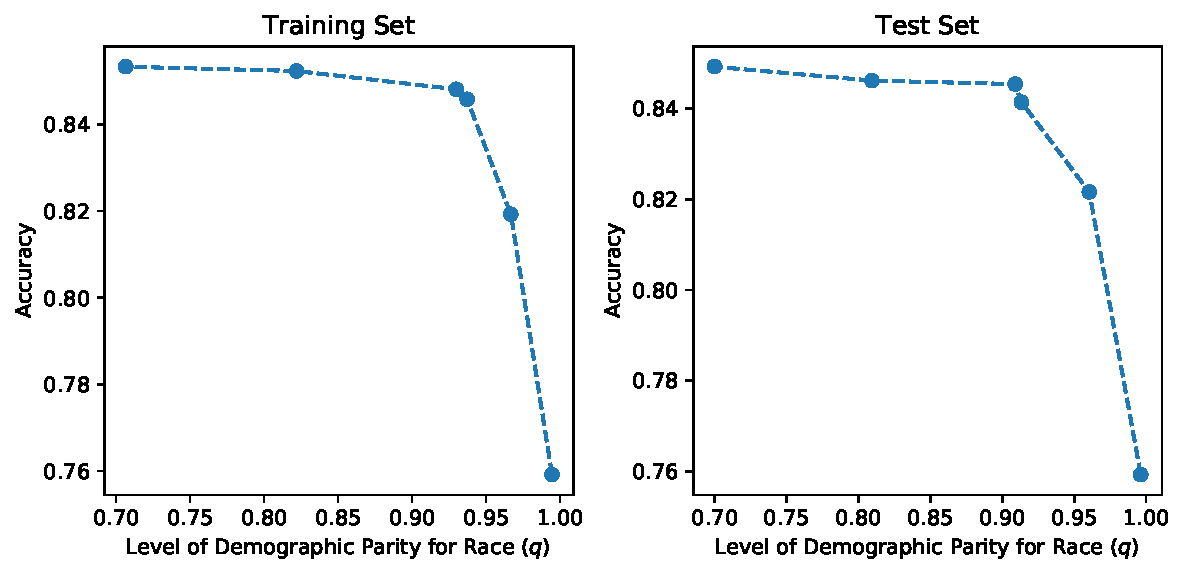
\includegraphics[width=\columnwidth]{img/boundary-tradeoff-race.pdf}}
\caption{Tradeoff between overall neural network accuracy and level of demographic parity for \emph{race} by varying regularization penalty $\lambda$ on the covariance between the distance to the decision boundary and sensitive attributes.  Results are given on the training set (left) and the test set (right).}
\label{boundary-fig-race}
\end{center}
\vskip -0.2in
\end{figure}

\begin{table}[ht]
\centering
\begin{tabular}{c|cc |cc} 
 \hline
 \hline
 $\lambda$ (for Race) & Train Acc & Train $q$ & Test Acc & Test $q$ \\ 
 \hline
 $3 \times 10^{-2}$ & 0.759 & \textbf{0.994} & 0.759 & \textbf{0.996}\\
 $1 \times 10^{-2}$ &0.819 & 0.967 & 0.822 & 0.960\\
$3 \times 10^{-3}$ & 0.846 & 0.937 & 0.841 & 0.913\\
$1 \times 10^{-3}$ &0.848 &0.930 &  0.845 &0.910 \\
$3 \times 10^{-4}$ & 0.852 & 0.822 & 0.846 & 0.810\\
$1 \times 10^{-4}$ & \textbf{0.853} & 0.707 & \textbf{0.849} & 0.700\\
 \hline
\end{tabular}
\caption{Numerical results of how accuracy and level of demographic parity change as functions of regularization parameter $\lambda$ for constraining prediction probabilities conditioned on \emph{race}.}  \label{boundary-table-race}
\end{table}

\begin{figure}[ht]
\vskip 0.2in
\begin{center}
\centerline{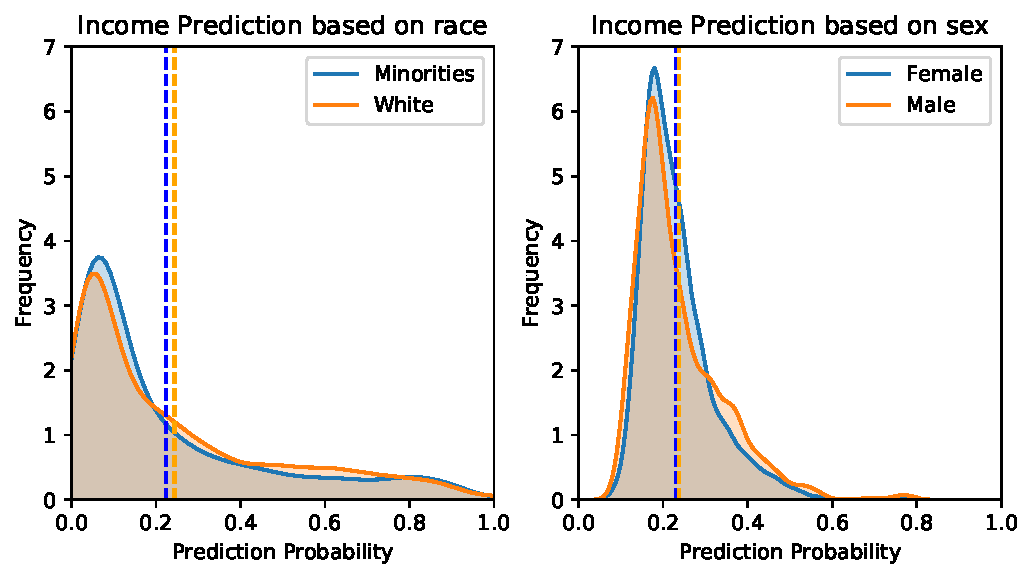
\includegraphics[width=\columnwidth]{img/boundary-bias.pdf}}
\caption{For the decision boundary-regularized neural network, fitted kernel density estimations of test set estimated probabilities that different races (left) and different sexes (right) make over 50K a year.  Dotted lines indicate the means of each distribution.}
\label{boundary-bias}
\end{center}
\vskip -0.2in
\end{figure}

\subsection{Regularizing with Adversarial Neural Networks}
Here, we adopt the model explained in Section \ref{sec:adversarial}. The predictor model $G$ is exactly equivalent to the vanilla neural network, so after pre-training, the results are equivalent to those described in Section \ref{vanilla-net}. The addition of the adversary $A$ and continued training leads to improvement in the fairness of the output predictions. In our experiments, we test the adversarial model for various values of $\alpha$ corresponding to how heavily the adversarial loss (ability to predict the sensitive attribute) is weighted with respect to the predictor loss. We test the values of $\alpha$ given in the following set: $\{1, 3, 10, 30, 100, 300 \}$. Note that since the adversary $A$ is able to predict all elements of $\bd z$, there is only 1 trial per $\alpha$ value. 

The resulting trends can be seen in Figures \ref{adv_fig_sex} and \ref{adv_fig_race}, with the statistics presented in Table \ref{adv-table}. Neither figure has as clear of a sharp bend as the figures for the previous method. Nevertheless, $\alpha=30$ appears to be a decent trade-off for both cases. For this value of $\alpha$, the resulting prediction distributions are seen in Figure \ref{adv-bias}. This graph is significantly different from Figure \ref{vanilla-nn} and shows significant improvement in equalizing the score distributions between individuals of different races or sexes. 

\begin{figure}[ht]
	\vskip 0.2in
	\begin{center}
		\centerline{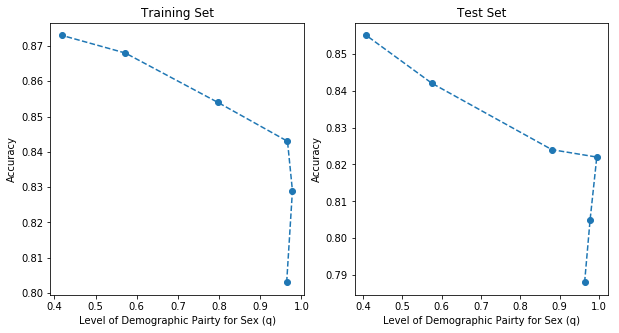
\includegraphics[width=\columnwidth]{img/adv_levels_sex.png}}
		\caption{Tradeoff between overall neural network accuracy and level of demographic parity for \emph{sex} by varying weight on adversarial loss $\alpha$. Results are given on the training set (left) and the test set (right).}
		\label{adv_fig_sex}
	\end{center}
	\vskip -0.2in
\end{figure}

\begin{figure}[ht]
	\vskip 0.2in
	\begin{center}
		\centerline{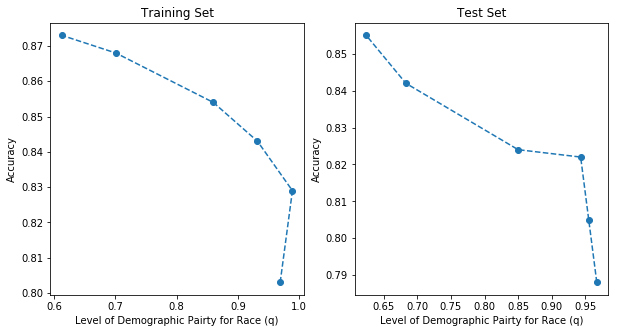
\includegraphics[width=\columnwidth]{img/adv_levels_race.png}}
		\caption{Tradeoff between overall neural network accuracy and level of demographic parity for \emph{race} by varying weight on adversarial loss $\alpha$. Results are given on the training set (left) and the test set (right).}
		\label{adv_fig_race}
	\end{center}
	\vskip -0.2in
\end{figure}

\begin{table}[!ht]
	\centering
	\begin{tabular}{c|ccc |ccc} 
		\hline
		\hline
		$\alpha$ & \shortstack{Train \\ Acc}  & \shortstack{Train  $q$ \\ Race} & \shortstack{Train  $q$ \\ Sex} & \shortstack{Test \\ Acc} & \shortstack{Test $q$ \\ Race} & \shortstack{Test $q$ \\ Sex} \\ 
		\hline
		300 & 0.803 & 0.969 & 0.964 & 0.788 & \textbf{0.967} & 0.963 \\ 
		100 & 0.829 & \textbf{0.989} & \textbf{0.978} & 0.805 & 0.955 & 0.977 \\
		30 & 0.843 & 0.932 & 0.966 & 0.822 & 0.943 & \textbf{0.994} \\
		10 & 0.854 & 0.860 & 0.797 & 0.824 & 0.850 & 0.880 \\
		3 & 0.868 & 0.701 & 0.572 & 0.842 & 0.683 & 0.575 \\ 
		1 & \textbf{0.873} & 0.613 & 0.418 & \textbf{0.855} & 0.624 & 0.408 \\
		\hline
	\end{tabular}
	\caption{Numerical results of how accuracy and level of demographic parity change as functions of regularization parameter $\alpha$ for adversarial models.} 
	\label{adv-table}
\end{table}

\begin{figure}[ht]
	\vskip 0.2in
	\begin{center}
		\centerline{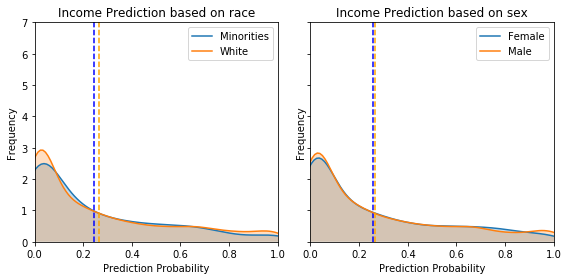
\includegraphics[width=\columnwidth]{img/adv_end.png}}
		\caption{For the adversarial neural network approach, fitted kernel density estimations of test set estimated probabilities that different races (left) and different sexes (right) make over 50K a year.  Dotted lines indicate the means of each distribution.}
		\label{adv-bias}
	\end{center}
	\vskip -0.1in
\end{figure}

\section{Discussion and Conclusion}
From the results, both methods clearly showed significant progress in improving the demographic parity relative to the vanilla neural network model. The plots showing the score distributions highlighted how the predictions for different races or sexes are similar after the application of these methods. Furthermore, using the statistics from the tables, it was clear that the methods achieve the $q \geq 0.8$ threshold that is important in legal contexts to create defensible models.

In light of these results, there are many directions for future work. First, one could test these results on other real-world datasets to explore how effective these methods are. In addition, the results from this paper were generally empirical. Both methods were able to improve $q$ scores without forsaking significant accuracy. It would be interesting to provide theoretical bounds for when a certain method will work and bound the loss in accuracy to achieve demographic parity. Finally, as mentioned in the introduction, demographic parity is only one definition of fairness of the more than twenty within literature. Further work could test the impact of these methods on other definitions and explore if they can be extended to meet multiple definitions of fairness.

\bibliographystyle{icml2019}
\bibliography{example_paper.bib}

\end{document}


% This document was modified from the file originally made available by
% Pat Langley and Andrea Danyluk for ICML-2K. This version was created
% by Iain Murray in 2018, and modified by Alexandre Bouchard in
% 2019. Previous contributors include Dan Roy, Lise Getoor and Tobias
% Scheffer, which was slightly modified from the 2010 version by
% Thorsten Joachims & Johannes Fuernkranz, slightly modified from the
% 2009 version by Kiri Wagstaff and Sam Roweis's 2008 version, which is
% slightly modified from Prasad Tadepalli's 2007 version which is a
% lightly changed version of the previous year's version by Andrew
% Moore, which was in turn edited from those of Kristian Kersting and
% Codrina Lauth. Alex Smola contributed to the algorithmic style files.
